\subsection*{Partie A}
Sur le graphique ci-dessous, on a tracé trois courbes $\mathcal{C}_{1}$\,, $\mathcal{C}_{2}$ et $\mathcal{C}_{3}$\,.

Les courbes correspondent aux représentations graphiques de trois fonctions définies sur $\R$ : une fonction $f$, sa dérivée $f'$ et sa dérivée seconde $f''$.

\begin{center}
	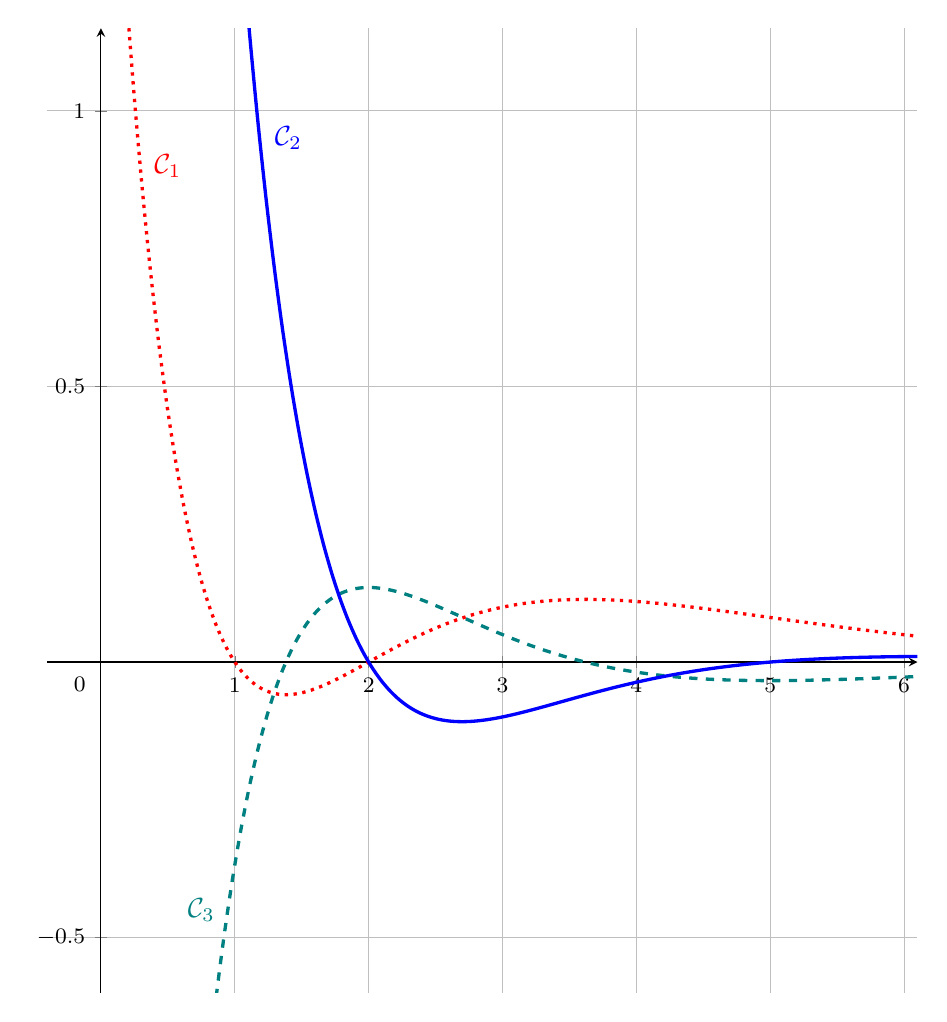
\begin{tikzpicture}
		\begin{axis}[x={17mm},y={70mm},
			xmin= -0.4,  xmax= 6.1, ymin = -.6, ymax=1.15,
			xtick distance=1, ytick distance=0.5,
			tick label style={font=\footnotesize}, grid=major, axis lines =center]
			\addplot [line width=1.2pt,color=red,smooth,samples=100,domain= 0:6.1,dotted]{exp(-x)*(x-1)*(x-2)};
			\addplot [line width=1.2pt,color=teal,smooth,samples=100,domain= 0:6.1,dashed]{exp(-x)*(-x*x+5*x-5)};
			\addplot [line width=1.2pt,color=blue,smooth,samples=100,domain= 0:6.1]{exp(-x)*(x*x-7*x+10)};
			\node[below left=2pt] at (0,0) {{\footnotesize 0}};
			\node[red] at(0.5,0.9) {$ \mathcal{C}_1 $};
			\node[blue] at(1.4,0.95) {$ \mathcal{C}_2 $};
			\node[teal] at(0.75,-0.45) {$ \mathcal{C}_3 $};
		\end{axis}
	\end{tikzpicture}
\end{center}

Associer chacune des fonctions $f$, $f'$ et $f''$ à sa courbe représentative. \emph{Aucune justification n'est attendue.}


\subsection*{Partie B}
On considère l'équation différentielle $(E)$ définie par $y'+y=(2 x-3) \e^{-x}$ où $y$ est une fonction de la variable réelle $x$.

\begin{enumerate}
	\item On considère la fonction $g$ définie sur $\R$ par
	\[g(x)=\left(x^{2}-3 x\right) \e^{-x}\]

	Démontrer que la fonction $g$ est une solution particulière de l'équation différentielle $(E)$.

	\item Déterminer l'ensemble des solutions de l'équation différentielle \quad $y'+y=0$.

	\item En déduire l'ensemble des solutions de l'équation différentielle $(E)$.

	\item Déterminer la solution $f$ de l'équation différentielle $(E)$ telle que \quad $f(0)=2$.
\end{enumerate}

\subsection*{Partie C}
On considère la fonction $f$ définie sur $\R$ par
\[f(x)=\e^{-x}\left(x^{2}-3 x+2\right)\]

et on note $\mathcal{C}_{f}$ sa courbe représentative dans un repère orthogonal.

\begin{enumerate}
	\item Étudier le signe de la fonction $f$ sur $\R$.

	\item \begin{enumerate}
		\item Déterminer la limite de la fonction $f$ en $-\infty$.

		\item Déterminer la limite de la fonction $f$ en $+\infty$.
	\end{enumerate}

	\item On note I l'intégrale définie par :
	\[I=\int_{0}^{1} f(x) \d x\]

	\begin{enumerate}
		\item À l'aide de deux intégrations par parties successives, démontrer que \quad $I=1-\dfrac{1}{\e}$.

		\item Interpréter graphiquement ce résultat.
	\end{enumerate}
\end{enumerate}

\subsection*{Partie D}
On considère un réel $a$.

On note $\left(T_{a}\right)$ la tangente à la courbe $\mathcal{C}_{f}$ au point d'abscisse $a$.

\begin{enumerate}
	\item Démontrer que le point d'intersection de la tangente $(T_{a})$ et de l'axe des ordonnées a pour ordonnée
	\[\left(a^{3}-4 a^{2}+2 a+2\right) \e^{-a}\]

	\item Déterminer le nombre de tangentes à la courbe $\mathcal{C}_{f}$ passant par l'origine du repère.

	Le candidat explicitera les étapes de la démarche utilisée.
\end{enumerate}
